\section{\Acl{NLP}}
\label{sec:nlp}

\subsection{An overview of \ac{NLP}}
\label{subsec:nlp-overview}
In an optimisation problem, the goal is to determine the minimum\footnote{
    In certain applications, the interest is actually in finding the maximum of
    a function. However, it is trivial to transform a maximisation problem into
    a minimisation problem by finding the minimum of negative of the function.
}
of a function $\Fth: \mathbb{R}^n \rightarrow \mathbb{R}, n \in \mathbb{N}$, often
called the \emph{cost function} or \emph{fidelity}.
This is typically with the goal of determining the argument $\bthstar$ at
which the minimum is found:
\begin{equation}
    \bthstar = \argmin_{\bth \in \mathbb{R}^n} \Fth.
    \label{eq:minF}
\end{equation}
The above problem is \emph{unconstrained}, as there are no limitations that the
parameter vector is subjected to. Unless $\Fth$ has particular properties, such
as convexity\footnote{
    A convex function is one such that a line segment through any two points of
    the function lies above it.
}, it is generally only possible to determine a \emph{local minimum},
rather than a \emph{global minimum} for high-dimensionality problems such as
the one of interest here. $\bthstar$ is a local
minimiser of $\Fth$ if there is a \emph{neighbourhood} $V \ni \bthstar$ for which
\begin{equation}
    \Fthstar \leq \Fth\ \forall \bth \in V.
  \label{def:local-minimiser}
\end{equation}
$V \subset \mathbb{R}^n$ is a continuous space such that one can move some
amount in any direction away from $\bthstar$ and still be in $V$.
Key to \ac{NLP} are the \emph{necessary conditions}, which define whether a
given vector $\bth$ is a local minimum of the fidelity.
The \emph{first necessary condition} states
that if $\Fth$ is continuously differentiable, and $\bthstar$ is a local extremum\footnote{
    ``Extremum'' is used here instead of ``minimum'', as the first necessary
    condition applies to maxima of a function as well as minima.
} of $\Fth$, then the gradient vector $\bdgthstar \coloneq \nabla \Fthstar$ is the
zero vector:
\begin{equation}
    \bdgthstar = \symbf{0} \in \mathbb{R}^n
\end{equation}
The \emph{second necessary condition} subsequently states that
if $\Fth$ and $\bdgth$ are continuously differentiable, and $\bthstar$ is a
local minimiser of $\Fth$, then the Hessian matrix $\bdHthstar \coloneq
\nabla^2 \Fthstar$ is positive semidefinite, i.e.
\begin{equation}
  \symbf{v}^{\mathrm{T}} \bdHthstar \symbf{v} \geq 0\ \forall \symbf{v} \in \mathbb{R}^n.
\end{equation}
Furthermore, it is a \emph{unique} local minimiser if the \emph{second-order
sufficient condition} is also satisfied, i.e. that the Hessian is positive
definite:
\begin{equation}
    \symbf{v}^{\mathrm{T}} \bdHthstar \symbf{v} > 0\ \forall \symbf{v} \in \mathbb{R}^n.
\end{equation}

A plethora of approaches have been established to determine local minima of
scalar functions. One of the better-known strategies is \emph{Newton's method},
in which a quadratic approximation of the fidelity is considered.
For a given iteration $k \in \mathbb{N}_0$, the fidelity is approximated using
\begin{equation}
    \FQth =
        \Fthk +
        \symbf{h}\T \bdgthk +
        \tfrac{1}{2} \symbf{h}^{\mathrm{T}} \bdHthk \symbf{h},
    \label{eq:quad-approx}
\end{equation}
where $\symbf{h} = \bth - \bthk$.  An updated prediction of the parameter
vector is derived by finding the minimum of this quadratic approximation:
\begin{gather}
    \frac{\partial \Fth}{\partial \symbf{h}} =
        \bdgthk + \bdHthk \symbf{h} \notag\\
    \implies 0 = \bdgthk + \bdHthk \left(\bthkplusone - \bthk\right) \notag\\
    \therefore\ \bthkplusone =
        \bthk - \bdHthk^{-1}
        \bdgthk.\label{eq:newton-update}
\end{gather}
This process is repeated, until the convergence criterion as been met:
\begin{equation}
    \left\lVert \bdgthk \right\rVert \leq \epsilon.
\end{equation}
The convergence threshold $\epsilon > 0$ can be tuned based on the desired
accuracy of the result.
\Cref{eq:newton-update} tends not to be used as the update formula in real
optimisation problems; one of the major downsides of the Newton update is the
possibility that is not a minimising update if the Hessian is not positive
definite. Two primary strategies have emerged which are typically used instead:
\begin{itemize}
    \item \emph{Line search methods}\cite[Chapter 3]{Nocedal2006} determine an
        appropriate direction $\symbf{p}^{(k)}$ along which the updated
        parameter vector is sourced.  After this, an appropriate step length
        $\alpha^{(k)}$ is determined\,---\,typically in an efficient, though not
        optimal manner\,---\,leading to $\bthkplusone = \bthk - \alpha^{(k)}\symbf{p}^{(k)}$.
    \item \emph{Trust region methods}\cite[Chapter 4]{Nocedal2006} define a
        radius $\Updelta^{(k)} > 0$, and determine the minimum of
        \cref{eq:quad-approx} subject to the constraint that
        $\left\lVert\symbf{h}\right\rVert \leq \Updelta^{(k)}$.
\end{itemize}
A trust region method is applied in this work, and as such further
consideration of it will now be made.

\begin{algorithm}
    \caption[
        Nonlinear programming routine employed in this work.
    ]
    {
        Nonlinear programming routine employed in this work. This makes use of
        Algorithms 4.1 \& 7.2 in \cite{Nocedal2006}, with a extra check
        inserted to deal with any negative-amplitude oscillators which may be
        generated as the routine evolves
        (\crefrange{state:neg-amp-start}{state:neg-amp-end}).
    }
    \label{alg:nlp}
    \begin{algorithmic}[1]
        \Procedure {NLP}{$\bY \in \mathbb{C}^{\None \times \cdots \times \ND}, \bthzero \in \mathbb{R}^{2(D + 1)M}$}
            \State $\trustradius{0} \gets \nicefrac{1}{10} \left\lVert \bdgthzeroY \right\rVert$;
            \State $\trmax \gets 16 \trustradius{0}$;
            \For {$k = 0, 1, \cdots $}
            \State $\symbf{p}^{(k)} \gets \textsc{SteihaugToint}\left(\symbf{Y}, \symbf{\theta}^{(k)}, \trustradius{k}\right)$;
                \Comment{See \cref{alg:steihaug-toint}}
                \State $\rho^{(k)} \gets
                    \frac
                        {\Fphithk - \Fphithkpk}
                        {\FphiQthk - \FphiQthkpk}$;
                \If {$\rho_k < \nicefrac{1}{4}$}
                \label{state:decrease-tr-start}
                \State $\trustradius{k+1} \gets \nicefrac{1}{4} \trustradius{k}$;
                    \label{state:decrease-tr-end}
                    \ElsIf {$\rho_k > \nicefrac{3}{4}$ \textbf{ and } $\left\lVert \symbf{p}^{(k)} \right\rVert = \trustradius{k}$}
                \label{state:increase-tr-start}
                \State $\trustradius{k+1} \gets \min\left(2 \trustradius{k}, \trmax\right)$;
                    \label{state:increase-tr-end}
                \Else
                \State $\trustradius{k+1} \gets \trustradius{k}$;
                \EndIf
                \If{$\rho^{(k)} > \nicefrac{3}{20}$}
                \label{state:large-rho-start}
                    \State $\bthkplusone \gets \bthk + \symbf{p}^{(k)}$;
                    \label{state:large-rho-end}
                \Else
                \label{state:small-rho-start}
                    \State $\symbf{\theta}^{(k+1)} \gets \symbf{\theta}^{(k)}$;
                    \label{state:small-rho-end}
                \EndIf
                \If{$k \bmod 25 = 0 \textbf{ and } \symbf{\theta}^{(k+1)}$ contains negative amplitudes}\label{state:neg-amp-start}
                    \State $\symbf{\theta}^{(0)} \gets \symbf{\theta}^{(k+1)}$ with negative-amplitude oscillators removed;
                    \State $\symbf{\theta}^{(*)}, \symbf{\epsilon}^{(*)} \gets \operatorname{NLP}\left(\symbf{Y}, \symbf{\theta}^{(0)}\right)$;
                \EndIf\label{state:neg-amp-end}
                \If{$\left\lVert \bdgthkplusone \right\rVert < \num[print-unity-mantissa=false]{1e-8}$}
                    \State \textbf{break};
                \EndIf
            \EndFor
            \State $\symbf{\theta}^{(*)} \gets \symbf{\theta}^{(k+1)}$
            \State $\symbf{\epsilon}^{(*)} \gets
                \sqrt{
                    \frac
                    {
                        \Fthstar \diag \left(
                            \left[\bdHthstar\right]^{-1}
                        \right)
                    }
                    {(\None \cdots \ND) - 1}
                }$
            \State \textbf{return} $\symbf{\theta}^{(*)}, \symbf{\epsilon}^{(*)}$;
        \EndProcedure
    \end{algorithmic}
\end{algorithm}
The structure of a typical trust region method is presented in
\cref{alg:nlp} (ignoring \crefrange{state:neg-amp-start}{state:neg-amp-end}, which is a custom addition,
see \cref{subsec:phase-variance}). An initial radius for the trust region
$\trustradius{0}$ is defined, along with a maximum permitted radius
$\trmax$, to ensure that excessively adventurous steps do not take place.
For each iteration, a solution to the following sub-problem is sought:
\begin{equation}
    \begin{split}
        \bpk = \argmin_{\bp \in \mathbb{R}^{n}}
            \Fthk +
            (\bthk + \bp)\T \bdgthk +
            \tfrac{1}{2} (\bthk + \bp)\T \bdHthk (\bthk + \bp) \\
        \text{subject to } \left \lVert \bp \right \rVert \leq \trustradius{k}.
    \end{split}
\end{equation}
This sub-problem is not usually minimised exactly, but instead an efficient
means of determining a sufficiently good update is used.
Common approaches include computing the Cauchy point, the Dogleg
method, and a truncated conjugate-gradient
approach commonly called the \ac{ST} method\cite[Chapter 7]{Nocedal2006}.
The latter is employed in this work (see \cref{alg:steihaug-toint} and
\cref{lst:tr}). In the \ac{ST} approach, iterates of the conjugate-gradient
method\cite[Chapter 5]{Nocedal2006} are computed, either until an iterate which
is outside the trust region is computed, or negative curvature is discovered.

Once a provisional update $\bthkplusone = \bthk + \bpk$ is determined using the
\ac{ST} method, a metric is considered which indicates how well the
quadratic estimate agrees with the true value of the fidelity:
\begin{equation}
    \rho^{(k)} = \frac
        {\Fthk - \Fthkpk}
        {\FQthk - \FQthkpk}.
\end{equation}
$\rho^{(k)}$ is the ratio between the actual reduction of the fidelity caused
by taking the proposed step, and the predicted reduction based on the quadratic
model. If $\rho^{(k)}$ is sufficiently close to $1$, the quadratic model being
used to generate new iterates is deemed to be acting well enough to warrant
accepting the proposed update
(\cref{state:large-rho-start,state:large-rho-end}).
Furthermore, if $\rho^{(k)}$ is particularly close to 1, and the proposed
update is at the boundary of the trust radius, it is appropriate to enlarge the
radius of the trust region for the next iteration in an attempt to increase the
rate of convergence
(\cref{state:increase-tr-start,state:increase-tr-end}).
On the other hand, a small value of $\rho^{(k)}$ implies that the
quadratic model reflects the true fidelity poorly, such that the proposed
update should be rejected
(\cref{state:small-rho-start,state:small-rho-end}).
As well as this, the trust region's radius should be
decreased such that the model is more likely to behave faithfully
(\cref{state:decrease-tr-start,state:decrease-tr-end}). In general, the
thresholds which dictate whether to accept an update, and whether to adjust the
trust region radius are customisable. The hard-coded numerical values found in
\cref{alg:nlp} are the values used for the results presented in this work.

\subsection{Non-linear programming applied to FID estimation}
\begin{remark}
    \label{rem:norm-data}
    Prior to estimating the dataset, it is normalised, such that the signal
    actually under consideration is $\nicefrac{\bY}{\lVert \bY \rVert}$.
    To make the result reflect the unnormalised dataset, the estiamted
    amplitudes $\bdastar$ are multiplied by $\lVert \symbf{Y} \rVert$.
\end{remark}
Focus now turns to the specific problem of FID estimation using \ac{NLP}, for
which a general $D$-dimensional dataset will be considered. As establised in
\cref{sec:theory-outline}, the fidelity $\FthY : \mathbb{C}^{\None \times
\cdots \times \ND} \times \mathbb{R}^{2(1 + D)M} \rightarrow \mathbb{R}$ is
given by
\begin{equation}
    \FthY = \left \lVert \bY - \bXth \right \rVert^2.
    \label{eq:fidelity}
\end{equation}
The elements of the gradient vector $\bdgthY \in \mathbb{R}^{2(1+D)M}$ and
the Hessian matrix $\bdHthY \in \mathbb{R}^{2(1+D)M \times 2(1+D)M}$ are
derived by taking the first and second partial derivatives of the fidelity with
respect to the elements in $\bth$:
\begin{subequations}
    \begin{gather}
        g_i = -2 \Re
                \left\langle
                    \left(\bY - \bX\right),
                    \frac{\partial \bX}{\partial \theta_i}
                \right\rangle,
        \label{eq:grad} \\
        h_{i,j} = 2 \Re
            \biggl(
                \underbrace{
                    \left\langle
                        \frac{\partial \bX}{\partial \theta_i},
                        \frac{\partial \bX}{\partial \theta_j}
                    \right\rangle
                }_{\circled{1}}
                -
                \underbrace{
                    \left\langle
                        \left(\bY - \bX\right),
                        \frac{\partial^2 \bX}{\partial \theta_i \partial \theta_j}
                    \right\rangle
                }_{\circled{2}}
            \biggl),
            \label{eq:hess}
    \end{gather}
    \label{eq:fidelity-grad-hess}%
\end{subequations}
$\forall i,j \in \lbrace 1, \cdots, 2(1+D)M \rbrace$.
The complete set of first and second derivatives of a particular element of the
model $x \coloneq \xnonenD$, given by \cref{eq:x}, is as follows
$\forall m \in \lbrace 1, \cdots, M \rbrace$,
$\forall d, d^{\prime} \in \lbrace 1, \cdots, D \rbrace$:
\paragraph{First dreivatives}
\begin{subequations}
    \begin{gather}
        \xderiv{\theta_m} \equiv
            \xderiv{a_m} =
            \frac{x}{a_m},\\
        \xderiv{\theta_{m + M}} \equiv
            \xderiv{\phi_m} =
            \iu x,\\
        \xderiv{\theta_{m + (d + 1)M}} \equiv
            \xderiv{\fdm} =
            2 \pi \iu \Dtd \nd x,\\
        \xderiv{\theta_{m + (d + D + 1)M}} \equiv
            \xderiv{\etadm} =
            - \Dtd \nd x.
    \end{gather}
\end{subequations}
\paragraph{Second derivatives}
\begin{subequations}
    \begin{gather}
        \xderivtwosame{\theta_{m}} \equiv
            \xderivtwosame{a_m} =
            0,
            \label{eq:amp-second-deriv}\\
        \xderivtwodiff{\theta_{m}}{\theta_{m + M}} \equiv
            \xderivtwodiff{a_m}{\phi_m} =
            \frac{\iu x}{a_m},\\
        \xderivtwodiff{\theta_{m}}{\theta_{m + (d + 1)M}} \equiv
            \xderivtwodiff{a_m^{\vphantom{(d)}}}{\fdm} =
            \frac{2 \pi \iu \Dtd \nd x}{a_m},\\
        \xderivtwodiff{\theta_{m}}{\theta_{m + (d + D + 1)M}} \equiv
            \xderivtwodiff{a_m^{\vphantom{(d)}}}{\etadm} =
            \frac{-\Dtd \nd x}{a_m},\\
        \xderivtwosame{\theta_{m + M}} \equiv
            \xderivtwosame{\phi_m} =
            -x,\\
        \xderivtwodiff{\theta_{m + M}}{\theta_{m + (d + 1)M}} \equiv
            \xderivtwodiff{\phi_m^{\vphantom{(d)}}}{\fdm} =
            -2 \pi \Dtd \nd x,\\
        \xderivtwodiff{\theta_{m + M}}{\theta_{m + (d + D + 1)M}} \equiv
            \xderivtwodiff{\phi_m^{\vphantom{(d)}}}{\etadm} =
            -\iu \Dtd \nd x,\\
        \xderivtwodiff{\theta_{m + (d + 1)M}}{\theta_{m + (d^{\prime} + 1)M}} \equiv
            \xderivtwodiff{\fdm}{\fdmp} =
            -4\pi^2 \left(\Dtd \nd \right) \left(\Dtdp \ndp \right) x,\\
        \xderivtwodiff{\theta_{m + (d + 1)M}}{\theta_{m + (d^{\prime} + D + 1)M}} \equiv
            \xderivtwodiff{\fdm}{\etadmp} =
            -2 \pi \iu \left(\Dtd \nd \right) \left(\Dtdp \ndp \right) x,\\
        \xderivtwodiff{\theta_{m + (d + D + 1)M}}{\theta_{m + (d^{\prime} + D + 1)M}} \equiv
            \xderivtwodiff{\etadm}{\etadmp} =
            \left(\Dtd \nd \right) \left(\Dtdp \ndp \right) x,\\
        \xderivtwodiff{\theta_{i}}{\theta_{j}} =
            \xderivtwodiff{\theta_{j}}{\theta_{i}},
            \label{eq:symmetric-second-derivs}\\
        \xderivtwodiff{\theta_{i}}{\theta_{j}} = 0\ \text{ if not specified above.}
        \label{eq:zero-second-deriv}
    \end{gather}
\end{subequations}
\Cref{eq:zero-second-deriv} indicates that any second derivative
with respect to two parameters which do not belong to the same oscillator will
always be $0$. This, along with the symmetrical nature of the second
derivatives (\cref{eq:symmetric-second-derivs}) drastically reduces the
required number to explicitly compute, from $4 (1 + D)^2 M^2$ per data-point
to  $(1+D)\left(3 + 2D\right)M$. Finally, \cref{eq:amp-second-deriv}
indicates that another $M$ second derivatives do not need to be computed, as
they are always $0$. See \cref{tab:number-of-derivatives} for the total
number of derivatives that need to be computed for datasets with different
numbers of dimensions.
\begin{table}
    \begin{center}
        \begin{tabular}{ c c c }
            \toprule
            Dimensions &
                \raisebox{\depth}{\#} 1\textsuperscript{st} derivatives &
                \raisebox{\depth}{\#} 2\textsuperscript{nd} derivatives\\
            \midrule
            $1$ & $4M\None$ & $9M\None$\\
            $2$ & $6M\None\Ntwo$ & $20M\None\Ntwo$\\
            $3$ & $8M\None\Ntwo\Nthree$ & $35M\None\Ntwo\Nthree$\\
            $D$ &  $2(1 + D)M \mathfrak{N}$ &  $((1 + D)(3 + 2D) - 1)M \mathfrak{N}$\\
            \bottomrule
        \end{tabular}
    \end{center}
    \caption{
        The number of first and second derivatives that are necessary to
        compute the gradient vector and Hessian matrix of the fidelity for
        1- 2- and 3-dimensional datasets, as well as a general $D$-dimensional
        dataset.
    }
    \label{tab:number-of-derivatives}
\end{table}

\subsection{Approximating the Hessian}
Despite many of the model second derivatives being $0$, computation of those
that are not zero, and subsequently using these the form the Hessian matrix, is
often the most computationally expensive part of the optimisation.
Numerous optimisation problems exist where this is the case, and as such
there is considerable precedent for improving the efficiency of optimisation
algorithms by generating approximations of the Hessian which are less expensive.
Examples include the \ac{GN} method and \ac{LM} algorithm,
which are specifically for \ac{RSS} problems\cite[Chapter
10]{Nocedal2006}, as well as quasi-Newton methods such as the \ac{BFGS}
method\cite[Chapter 6]{Nocedal2006}.

The \ac{GN} and \ac{LM} approaches replace the true Hessian matrix at each
iteration with the following expression:
\begin{equation}
    h_{i,j} = 2 \Re
        \left\langle
            \frac{\partial \bX}{\partial \theta_i},
            \frac{\partial \bX}{\partial \theta_j}
        \right\rangle,
    \label{eq:hess-approx}
\end{equation}
i.e. term \circled{2} in \cref{eq:hess}, which involves the model second
derivatives, is neglected. All that needs to be generated is the Jacobian
$\symbf{J} = \nicefrac{\partial \bX}{\partial \bth}$. This can
bring a very large reduction in the computational cost, as no extra
derivatives need to be computed for the Hessian at all, since the Jacobian is
already required for generating the gradient vector.
In situations where the residuals between the data and model are small, term
\circled{1} will tend to dominate term \circled{2}, and as such these methods
often enjoy a convergence rate which is comparable to that of Newton's method
when close to local minima. Despite this, by invoking this approximation, the
rate of convergence, i.e. the number of iterations required to reach
$\bthstar$, tends to be adversely affected. See \cref{subsec:optim-vis} for an
example of this phenomenon.

\subsection{Estimation Errors}
\label{subsec:errors}
A measure of the degree of uncertainty in the parameter estimates can be obtained
by computing the \emph{standard errors} associated with the \ac{NLP} routine.
Standard errors are related  to the \emph{observed Fisher information matrix}
at convergence\cite[Section 2.7]{Pawitan2001}:
\begin{equation}
    \symbf{\epsilon}\left(\bthstar\right) = \sqrt{\diag\left(\symbf{I}\left( \bthstar \right)^{-1}\right)},
\end{equation}
where the observed Fisher Information matrix contains the negative partial second
derivatives of the log-likelihood with respect to $\bth$:
\begin{equation}
    \symbf{I}\left(\bth\right)_{i, j} =
        -\frac
        {\partial^2 \ell \left( \bdthY \right)}
        {\partial \theta_i \partial \theta_j}.
\end{equation}
Recalling the form of the log-likelihood given by \cref{eq:log-likeihood},
the elements of $\symbf{I}\left(\bth\right)$ are
\begin{equation}
    \symbf{I}\left(\bth\right)_{i, j} =
        -\frac{1}{\sigma^2}
        \Re
        \biggl(
            \left\langle
                \frac{\partial \bX}{\partial \theta_i},
                \frac{\partial \bX}{\partial \theta_j}
            \right\rangle
            -
            \left\langle
                \left(\bY - \bX\right),
                \frac{\partial^2 \bX}{\partial \theta_i \partial \theta_j}
            \right\rangle
        \biggl),
\end{equation}
which very closely resembles the Hessian of $\bth$:
\begin{equation}
    \symbf{I}\left(\bth\right)_{i,j} =
        \frac{1}{2 \sigma^2}
            \bdHth_{i,j}.
\end{equation}
The standard errors therefore take the form
\begin{equation}
    \symbf{\epsilon}\left(\bthstar\right) =
        \sqrt{
            2\sigma^2 \diag \left(
                \bdHthstar^{-1}
            \right)
        }.
\end{equation}
The mean and variance of the noise are $0$ and $2\sigma^2$, respectively,
leading to:
\begin{equation}
    2 \sigma^2 = \frac{1}{\mathfrak{N} - 1}
    \left\lVert \bW \right\rVert^2 =
    \frac{1}{\mathfrak{N} - 1} \left \lVert
        \bY - \bXthstar
    \right \rVert^2.
\end{equation}
Finally a useable expression for the standard errors is arrived at:
\begin{equation}
    \symbf{\epsilon}\left(\bthstar\right) =
        \sqrt{
            \frac
            {
                \Fthstar \diag \left(
                    \bdHthstar^{-1}
                \right)
            }
            {\mathfrak{N} - 1}
        }
\end{equation}

\subsection{Visualisation of a simple example}
\label{subsec:optim-vis}
\begin{figure}
    \centering
    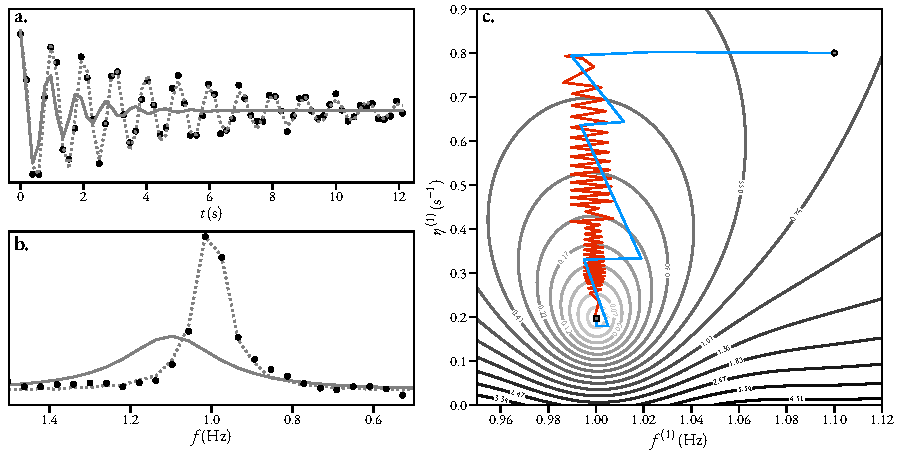
\includegraphics{optimisation_visualisation/optimisation_visualisation.pdf}
    \caption[
        A visualisation of the trajectory of a 2-parameter optimisation
        involving a simulated \acs{FID} comprising a single signal.
    ]
    {
        A visualisation of the trajectory of a 2-parameter optimisation
        involving a simulated \acs{FID} comprising a single signal.
        \textbf{a.} \& \textbf{b.} Representations of the signal in
        the time domain and Fourier domain, respectively.
        Black dots: the signal to be estimated $\by$.
        Solid grey line: the model generated
        using the initial guess $\bx \left( \bthzero \right)$.
        Dotted grey line: the model generated using the optimised result, $\bx
        \left( \bthstar \right)$.
        \textbf{c.} A contour plot of the fidelity.
        Blue line: the trajectory of the parameter vector with the true
        Hessian matrix used in computing each update.
        Red line: the analogous trajectory using the Hessian approximation
        in place of the true Hessian.
    }
    \label{fig:optim-vis}
\end{figure}
\Cref{fig:optim-vis} provides a visual example of the application of \ac{NLP}
to estimate a simulated \ac{1D} \ac{FID} comprising a single signal.
The FID was constructed using \cref{eq:general-fid} with $M=1$,
$N = 64$, $\fsw = \qty{5.2}{\hertz}$ ($\Dt \approx
\qty{0.192}{\second}$), and $\foff = \qty{0}{\hertz}$.
The signal was parameterised by $\bth \in \mathbb{R}^4$ comprising $a=1$,
$\phi=\qty{0}{\radian}$, $f=\qty{1}{\hertz}$, $\eta=\qty{0.2}{\per\second}$.
\ac{AWGN} was added to the \ac{FID} to give it \iac{SNR} of approximately
\qty{10}{\deci\bel}. As the visualisation of 5D space is beyond the scope of
this work, only two parameters, the frequency and damping factor, were optimised
from an initial guess $\bthzero$; the amplitude and phase were fixed to
their true values throughout. The initial guess comprised a frequency of
\qty{1.1}{\hertz}, and a damping factor of \qty{0.8}{\per\second}, with the
solid grey lines in panels a \& b denoting the model generated in the time- and
Fourier-domains, respectively. $\bthzero$ was subjected to \ac{NLP} twice. In
the first instance, the exact Hessian matrix, given by \cref{eq:hess} was used
in order to compute each update step, while in the second the Hessian
approximation given by \cref{eq:hess-approx} was used. The initial
radius of the trust region was set to $\nicefrac{1}{10}$ of the gradient norm
($\approx 0.3$), which has a precedent in the literature\cite{Gould2005}. The
trajectories of the parameter vector are denoted by coloured lines in panel c.
In both cases, the \ac{NLP} routine successfully converged at a result $\bthstar$
in agreement with the true frequency and damping factor used to construct the
\ac{FID}. However, it is clear that using the true Hessian matrix (blue)
led to a far better rate of convergence compared with the
approximated analogue (red), which exhibited ``zig-zagging''\footnote{
    This phenomenon is often seen in gradient descent methods, in which each
    update occurs along the opposite direction to the gradient.
}.
14 iterations were required to reach the
convergence criterion $\epsilon \leq \num[print-unity-mantissa=false]{1e-8}$
when the true Hessian was used, while 81 were required for the approximated
case. Despite being an anecdotal example, this highlights that use of the true
Hessian matrix tends to allow a better rate of convergence. However, for
\acp{FID} comprising many signals and far more points, the approximated form
often requires a shorter time to converge overall; the cost of computing the
second derivatives required for the true Hessian becomes incredibly expensive,
as will become clear in \cref{sec:profiling}.

\subsection{Phase Variance Minimisation}
\label{subsec:phase-variance}
An \ac{NLP} procedure tasked with minimising the discrepancy between a model
and the observed data is well-suited to produce an accurate holistic
representation of the data, assuming a sufficiently large
model order is used. However, as with many inverse problems, \ac{FID}
estimation is \emph{ill-posed}\cite{Kabanikhin2008}; there
is conceivably a large set of parameter vectors which will achieve a good
\ac{RSS} fit.
An added dimension of difficulty exists for \ac{FID} estimation, as the
number of parameters to be estimated is not hard-coded since the model order
is commonly not known.
It is desirable to produce an estimate which not only achieves a good fit to
the data, but which is also in agreement with the process underpinning the
observation. It is for this reason that iterative procedures typically require
significant quantities of prior knowledge\,---\,beyond basic assumptions of the
underlying model,\,---\,in order to produce meaningful estimation results.
This is also why they are often able to produce results which agree better with
a spectroscopist's conception of what the ``correct'' parameter estimate is,
relative to other methods where such detailed information is not exploited.

While the \ac{MPM} is often able to generate reasonable parameter estimates,
one particular feature has been noticed which is a common across
results: often, oscillators in the model exhibit ``spurious
phases''. As has been discussed (\cref{subsec:nmr-proc}),
signals in most \ac{NMR} experiments have phases which depend on their
resonance frequencies to first order. This is routinely corrected in
conventional \ac{NMR} spectral processing, such that all signals are adjusted to
acquire a phase of \qty{0}{\radian}. This feature of the dataset can be
exploited in order to overcome the aforementioned shortcoming of the \ac{MPM},
through appropriate adjustment of the \ac{NLP} routine. Assuming that
the data has been phase corrected\footnote{
    Rather than rely on the data being phase-corrected, one could envisage
    replacing the phase variance with a term which guides the
    oscillators to adopt a first-order phase relationship. The reason why the
    phase variance has been chosen is two-fold: (i) Applying phase-correction
    to \ac{NMR} data is straightforward and can be automated,
    meaning the user would experience minimal burden. (ii) As will be discussed
    in \cref{sec:filtering}, it is beneficial to have a spectrum comprising
    pure absorption-mode Lorentzians in order to produce frequency-filtered
    ``sub-\acp{FID}'' from the original data, so the data being estimated will
    be phase-corrected anyway.
}, regularising the fidelity by incorporating the variance of oscillator
phases can lead to improved estimation results. Examples of
this principle will be provided later (\cref{sec:evaluation}).
The updated fidelity becomes
\begin{equation}
    \FphithY = \left \lVert \bY - \bXth \right \rVert^2 + \circvar,
    \label{eq:fidelity-phasevar}
\end{equation}
where $\circvar$ is the \emph{circular variance} of the oscillator phases.
\begin{remark}
    The inclusion of the phase variance into the fidelity is one of the
    motivating reasons for normalising the data prior to estimation (see
    \cref{rem:norm-data}). $\circvar$ is constrained to the interval $[0, 1]$.
    If the data were not normalised, it is likely that $\lVert \bY - \bX
    \rVert^2$ would dominate $\circvar$ in \cref{eq:fidelity-phasevar},
    such that the influence of the phase variance would be negligible.
\end{remark}

Oscillator phases are an example of a \emph{circular variable}, in that all
phases are wrapped within an interval of width
2$\pi$\,\unit{\radian}. Given an
unconstrained (unwrapped) phase $\widetilde{\phi} \in \mathbb{R}$, the
corresponding wrapped phase $\phi \in \left( -\pi, \pi \right]$ is given by
\begin{equation}
    \phi = \left(\left(\widetilde{\phi} + \pi\right) \bmod 2 \pi\right) - \pi.
    \label{eq:phase_wrap}
\end{equation}
This makes the conventional (linear)
definition of variance, given by
\begin{subequations}
    \begin{gather}
        \Var_{\shortmid}\hspace*{-3pt}\left(\symbf{\phi}\right) =
            \frac{1}{M} \sum_{m=1}^{M} \left(\phi_m - \mu\left(\symbf{\phi}\right)\right)^2, \\
        \mu\left(\symbf{\phi}\right) = \frac{1}{M} \sum_{m} \phi_m,
    \end{gather}
\end{subequations}
unsuitable for phases. Consider as a simple example a scenario
where there are two oscillators with phases $\widetilde{\bdphi} = \left[ \pi +
\delta\:\:\pi - \delta \right]\T$ for some small $\delta$.
The phase variance is expected to be small as the phases are similar.
However, with the inclusion of wrapping through application of
\cref{eq:phase_wrap}, these phases would actually be set to $\bdphi = \left[
    -\pi
+ \delta\:\:\pi - \delta \right]\T$, and the linear phase
variance would be large. It is therefore apparent that a definition of variance
which accounts for the periodicity of the phases is needed. The \emph{circular
variance} is given by\cite[Chapter 3]{Fisher1993}
\begin{subequations}
    \begin{gather}
        [0, 1] \ni \circvar = 1 - \frac{R}{M},\\
        R = \sqrt{c_{\Sigma}^2 + s_{\Sigma}^2}, \\
        c_{\Sigma} = \sum_{m} \cos \phi_m, \\
        s_{\Sigma} = \sum_{m} \sin \phi_m.
    \end{gather}
\end{subequations}
$R$ is the length of the resultant vector produced by summing $M$ unit vectors
with the angles given by $\bdphi \in \mathbb{R}^M$. In the case that all the vectors have the
same angle, $R=M$, leading to the variance being $0$ as expected. At the other
extreme, with $M$ vectors uniformly separated about the unit circle\,---\,such
that there is an angle of $\nicefrac{2 \pi}{M - 1}$\,\unit{\radian} between all
pairs of adjacent vectors\,---\,the
vectors will perfectly cancel, leading to $R=0$. In this case, the maximum
variance of $1$ is obtained.
The first and second derivatives of the circular variance are required for
the computation of the gradient vector and Hessian matrix, through
\begin{subequations}
    \begin{gather}
        g_i = -2 \Re
                \left\langle
                    \left(\bY - \bX\right),
                    \frac{\partial \bX}{\partial \theta_i}
                \right\rangle
                + \frac{\partial \circvar}{\partial \theta_i} \\
        h_{i,j} = 2 \Re
            \biggl(
                    \left\langle
                        \frac{\partial \bX}{\partial \theta_i},
                        \frac{\partial \bX}{\partial \theta_j}
                    \right\rangle
                -
                \underbrace{
                    \left\langle
                        \left(\bY - \bX\right),
                        \frac{\partial^2 \bX}{\partial \theta_i \partial \theta_j}
                    \right\rangle
                }_{\parbox{6em}{\scriptsize{Neglected if approximation used}}}
            \biggl)
            + \frac{\partial^2 \circvar}{\partial \theta_i \partial \theta_j}.
    \end{gather}
\end{subequations}
The derivatives of the phase variance are given by:
\begin{subequations}
    \begin{gather}
        \frac{\partial \circvar}{\partial \theta_i} =
        \begin{cases}
            \frac{1}{RM}
            \left(
                c_{\Sigma} \sin \phi_{i-M} -
                s_{\Sigma} \cos \phi_{i-M}
            \right) & M \leq i < 2M\\
            0 & \text{otherwise}
        \end{cases}\\
        \frac{\partial^2 \circvar}{\partial \theta_i \partial \theta_j} =
        \begin{cases}
            \begin{split}
                \tfrac{1}{RM}\left[
                    \tfrac{1}{R^2}
                    \left(c_{\Sigma} \sin \phi_{i-M}  - s_{\Sigma} \cos \phi_{i-M} \right)^2 \right. \\
                    \left. + c_{\Sigma} \cos \phi_{i-M} + s_{\Sigma} \sin \phi_{i-M}
                    - 1
                \vphantom{\tfrac{1}{RM}}\right]
            \end{split}
            & M \leq i, j < 2M, i = j\\
            \begin{split}
                \tfrac{1}{RM}\left[
                    \tfrac{1}{R^2}
                    \left(c_{\Sigma} \sin \phi_{i-M} - s_{\Sigma} \cos \phi_{i-M} \right) \right.\\
                    \times \left(c_{\Sigma} \sin \phi_{j-M} - s_{\Sigma} \cos \phi_{j-M} \right) \\
                    \left. - \cos\left( \phi_{i-M} - \phi_{j-M} \right)
                    \vphantom{\tfrac{1}{R^2}}
                \right]
            \end{split}
            & M \leq i, j < 2M, i \neq j\\
            0 & \text{otherwise}
        \end{cases}
    \end{gather}
\end{subequations}

The phase variance-regularised fidelity (\cref{eq:fidelity-phasevar}) is
minimised according the unconstrained \ac{NLP} routine described above. It is
therefore possible for oscillators to acquire parameters which are unrealistic
as the optimiser evolves (see \cpageref{pg:param-constraints} for a description
of the sets that the parameters are expected to be in). With the inclusion of
the variance of oscillator phases, there are situations where oscillators
acquire negative amplitudes. Typically, this occurs when there are
oscillators in the \ac{MPM} result which start out with phases that are close
to $\qty{\pi}{\radian}$. By acquiring a negative amplitude, and a phase close to
\qty{0}{\radian}\,---\,the expected phase of most oscillators in the parameter
set\,---\,little change to the residual sum-of-squares term is made, while
reducing the value of $\circvar$. The presence of such oscillators is
undesirable, as they are spurious in the context of well-phased data. As a
result, the \ac{NLP} routine periodically checks for negative-amplitude oscillators
(\crefrange{state:neg-amp-start}{state:neg-amp-end} in \cref{alg:nlp}). After a
given number of iterations ($25$ is the value given in \cref{alg:nlp}, but this
can of course be adjusted), if any oscillators have acquired negative
amplitudes, these are purged, and the routine continues.
